\documentclass[hidelinks]{scrartcl}
\usepackage[final]{nips_2016}
\usepackage{amsmath, amsthm}
\usepackage{amssymb}
\usepackage{color, soul}
\usepackage[margin=0.5in]{geometry}
\usepackage{hyperref}
%% \usepackage[]{mcode}
\usepackage{cancel}
\usepackage{tabu}
\usepackage{colortbl}
\usepackage{graphicx}
\usepackage{subcaption}
\usepackage{verbatim}
\usepackage{tikz}
\usepackage{float}


\newcommand{\Lbf}[1]{{\noindent \Large{\textbf{#1}}}}
\newcommand{\Part}[1]{\vspace{1cm} {\LARGE\textbf{PART #1}}\\}


%opening
\title{HW3: Deep RL and Controls}



\author{Kenny Marino, Rick Goldstein, Brad Saund, Xiang Zhi Tan}

\begin{document}
\maketitle

%%%%%%%%%%%%%%%%%%%%%%%%%%%%%%%%%%%%%%
\section*{Problem 1}
\subsection*{LQR}
Table \ref{table:LQR_performance} reports the total reward and numbers of steps for each environment. The plots showing the control inputs and robots states are shown in figure \ref{fig:LQR_state}. 

\begin{table}[h]
	\centering
	\begin{tabular}{|l|c|c|}
		\hline	
		Environment Name & Total Reward & Number of Steps\\
		\hline
		TwoLinkArm-v0 & $-587.113158273954$ & 114 \\ 
		TwoLinkArm-limited-torque-v0 & $-8099.057755102057$ & 2383\\
		TwoLinkArm-v1 & $-3812.829669478557$ & 462 \\
		TwoLinkArm-limited-torque-v1 & $-3777.977482886332$ & 1176 \\		
		\hline
	\end{tabular}
	\\
	\captionof{table}{Total Reward and Number of Steps for LQR in different OpenAI Gym Environment}
	\label{table:LQR_performance}
\end{table}

\begin{figure}[H]
	\centering
    \begin{subfigure}[b]{0.45\textwidth}
        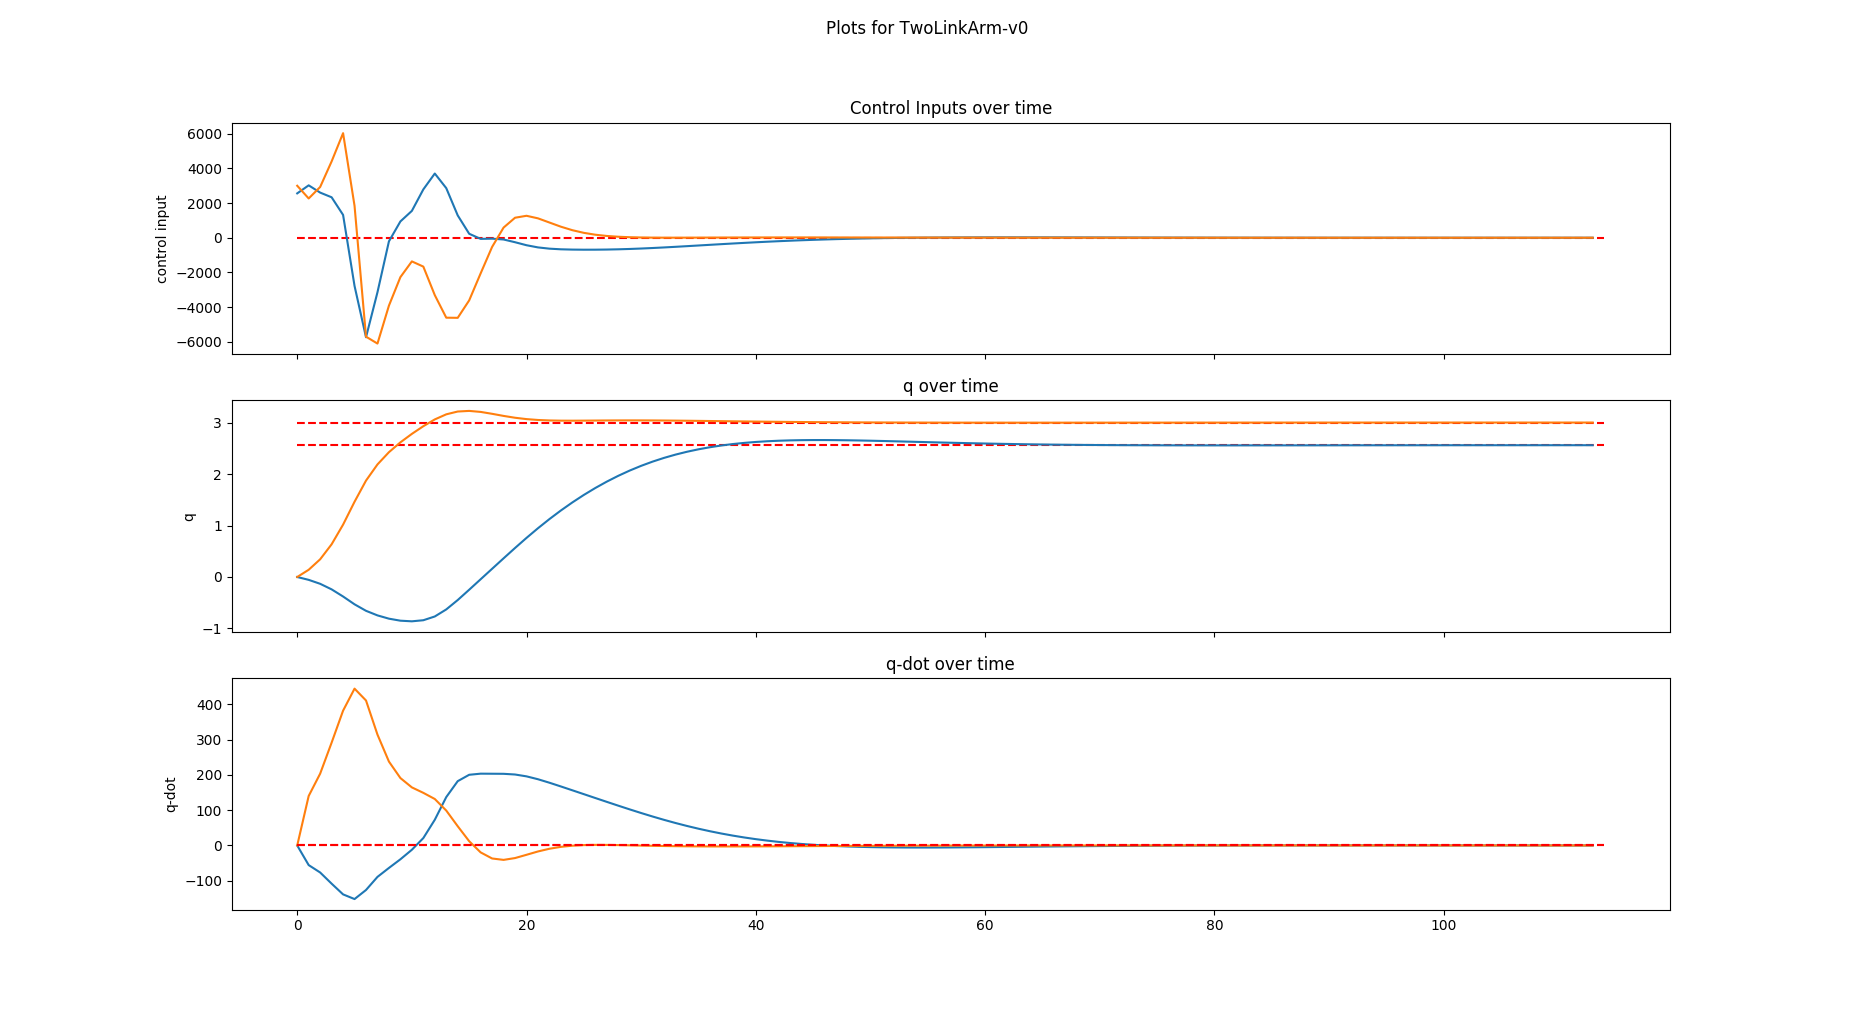
\includegraphics[width=\textwidth]{figures/twolinkarm-v0}
        \caption{TwoLinkArm-v0}
    \end{subfigure}
    \begin{subfigure}[b]{0.45\textwidth}
        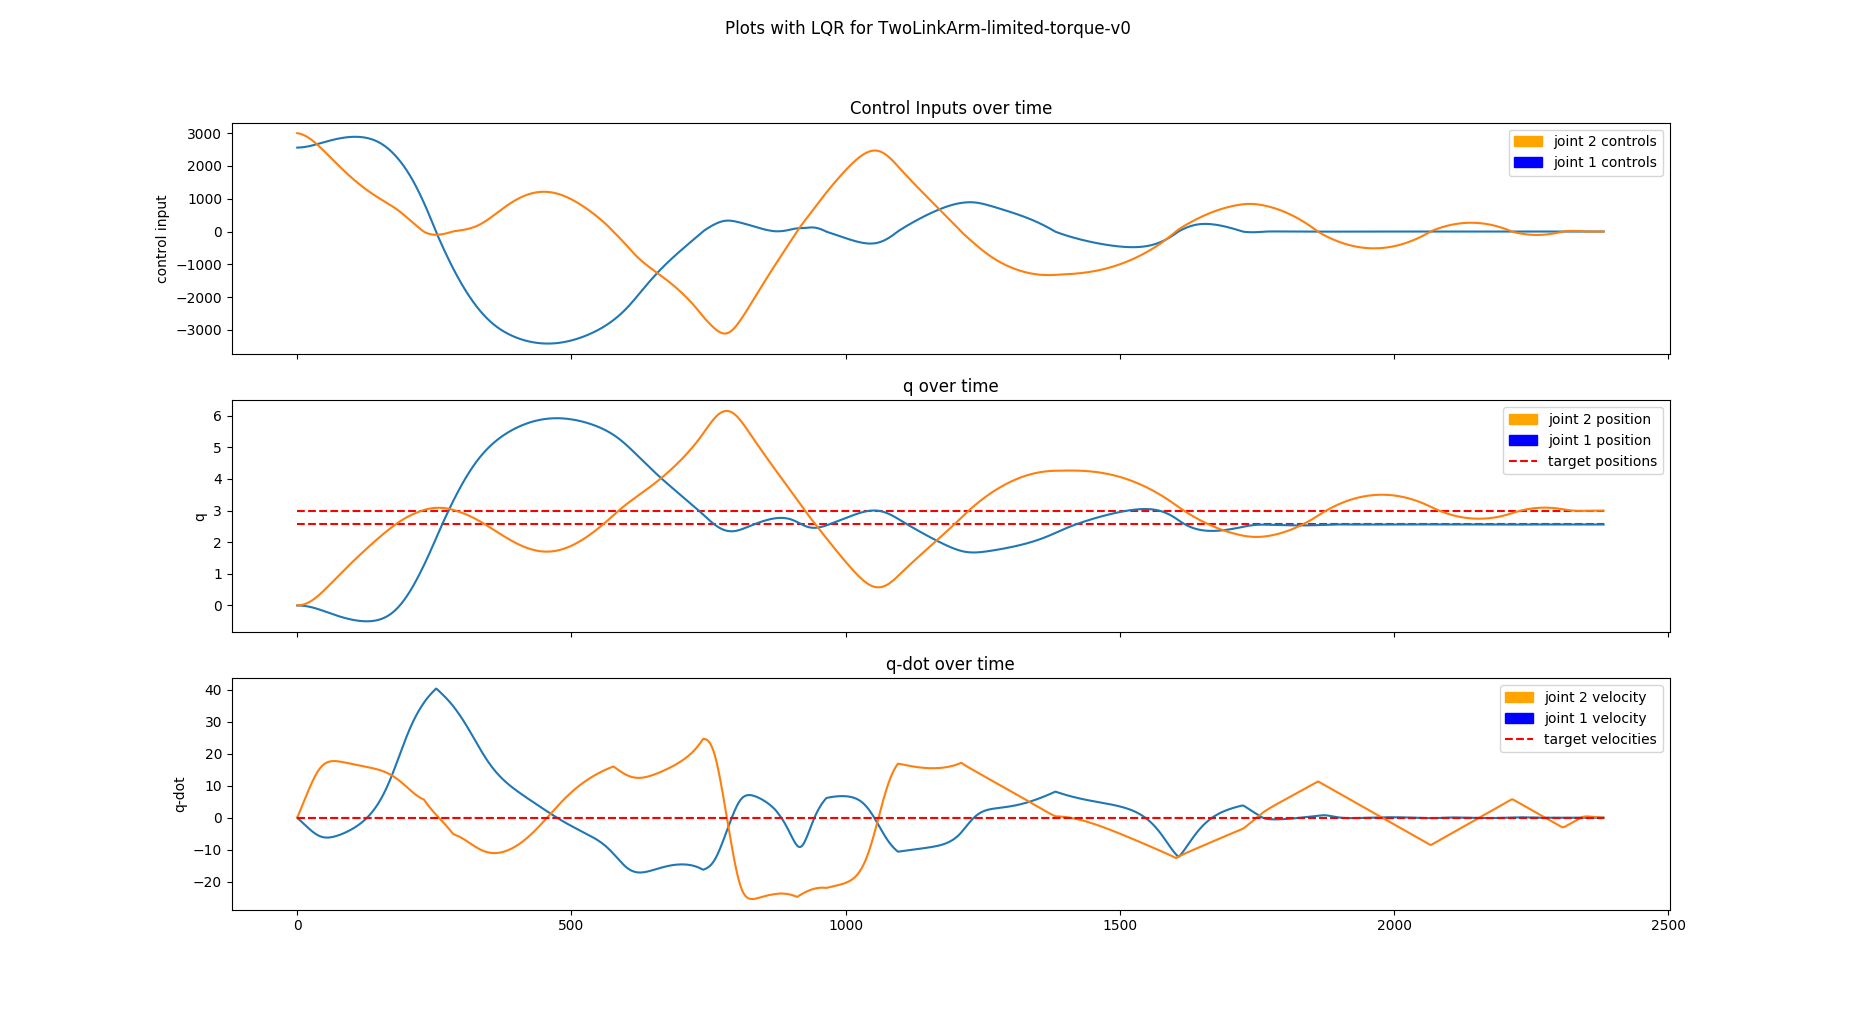
\includegraphics[width=\textwidth]{figures/twolinkarm-limited-v0}
        \caption{TwoLinkArm-limited-torque-v0}
    \end{subfigure}
    \\
     \begin{subfigure}[b]{0.45\textwidth}
        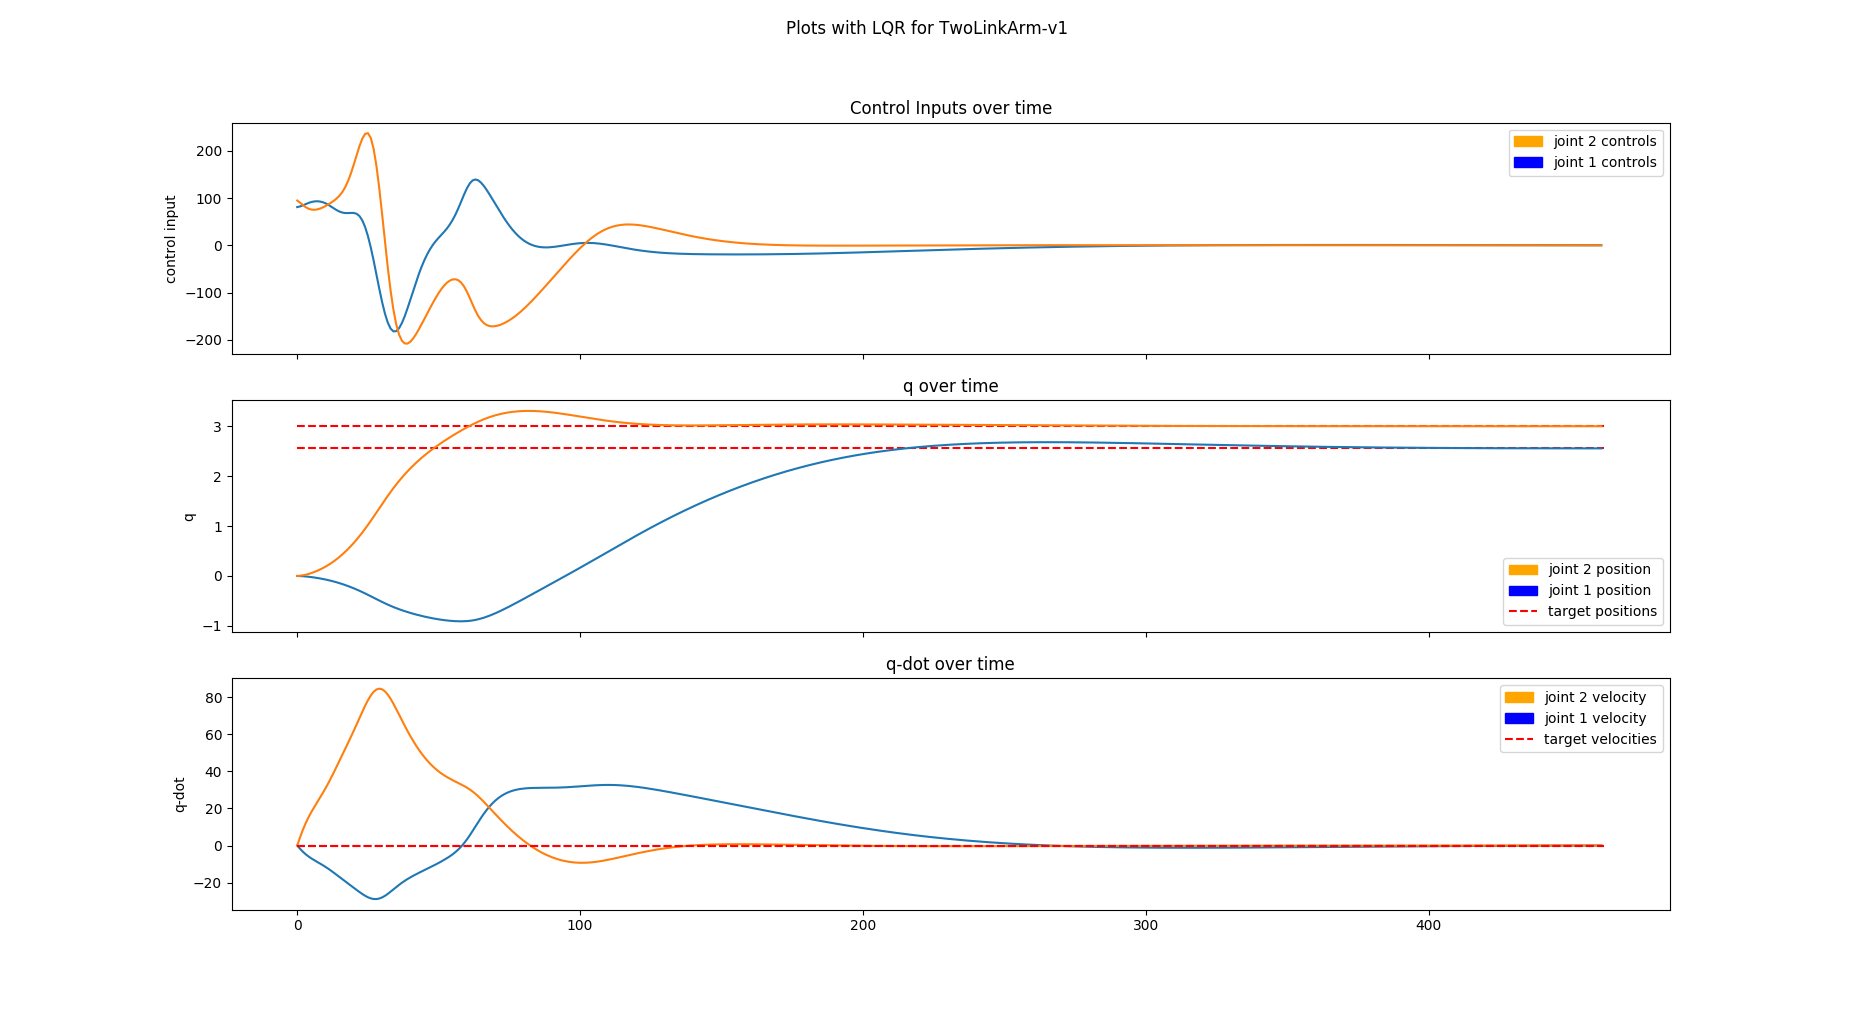
\includegraphics[width=\textwidth]{figures/twolinkarm-v1}
        \caption{TwoLinkArm-v1}
    \end{subfigure}
    \begin{subfigure}[b]{0.45\textwidth}
        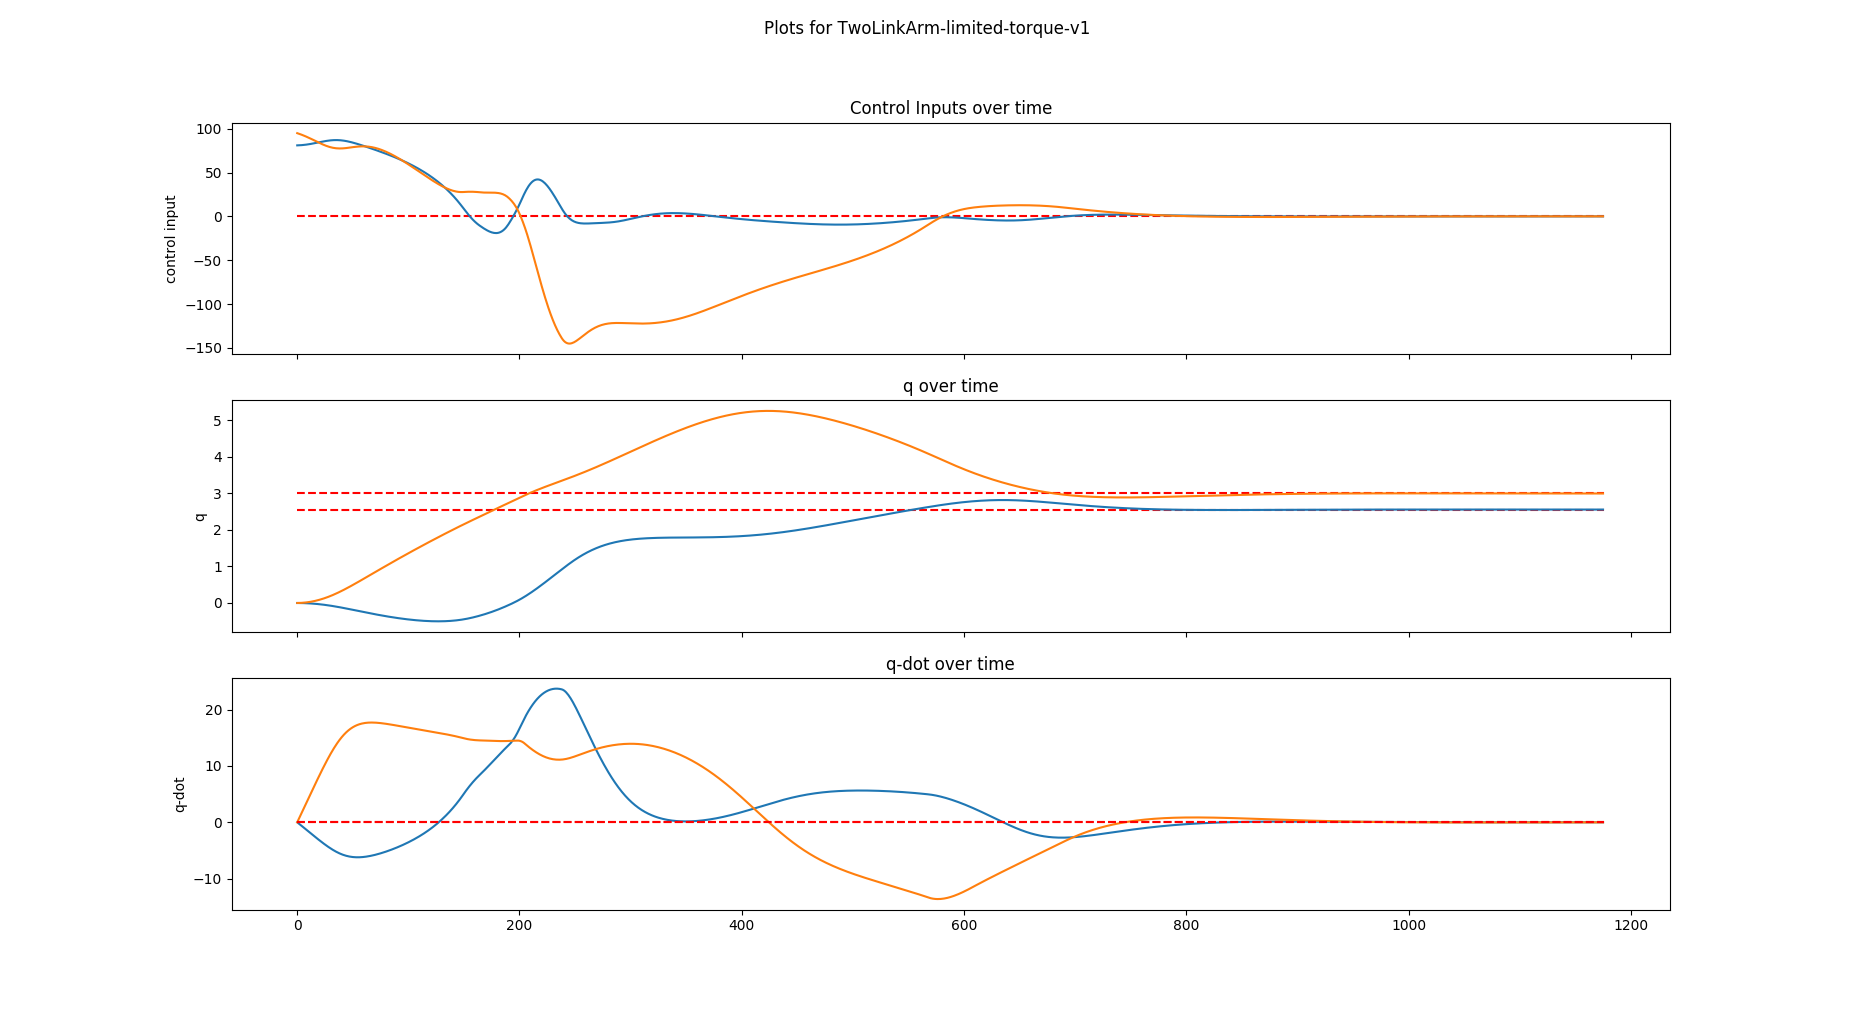
\includegraphics[width=\textwidth]{figures/twolinkarm-limited-v1}
        \caption{TwoLinkArm-limited-torque-v1}
    \end{subfigure}
    \caption{Control signals, robot arm state in different environment over time}\label{fig:LQR_state}
\end{figure}
\subsubsection*{Analysis}
Comparing \textit{TwoLinkArm-v0} and \textit{TwoLinkArm-limited-torque-v0}, we can observe that the agent in in textit{TwoLinkArm-limited-torque-v0} took significantly longer. This was because the arm can accelerate faster with larger torque inputs. The limit of $10$ in \textit{TwoLinkArm-limited-torque-v0} limited the acceleration of the arm and potential maximum velocity. We can observe this in the plots where the maximum velocity of \textit{TwoLinkArm-v0} was 400 compared to the maximum of 40 in \textit{TwoLinkArm-limited-torque-v0}. Because of the longer runtime, the agent incurred larger negative reward.\\
Comparing \textit{TwoLinkArm-v0} and \textit{TwoLinkArm-v1}, the biggest difference between these two condition was the maximum torque applied. The torques in \textit{TwoLinkArm-v0} peaked at 6000 compared to 200 in \textit{TwoLinkArm-v1}. This was because LQR optimized for the larger cost by large torques in \textit{TwoLinkArm-v1} and choose to minimize the torque applied.\\
When comparing \textit{TwoLinkArm-limited-torque-v1} and \textit{TwoLinkArm-limited-torque-v0}, again the biggest difference is the amount of torque applied by the agent. The agent in \textit{TwoLinkArm-limited-torque-v1} apply less torque because of the higher cost.

\subsection*{iLQR}
For our iLQR implemented, we followed the algorithm of Differential Dynamic Programming\footnote{https://en.wikipedia.org/wiki/Differential_dynamic_programming}. Our understanding is that iLQR is just a variant of DDP where the state function is linear and doesn't have 2nd derivatives. Our algorithm first do a 100 step look ahead with 100 iterations. We then apply those 100 control signals. If the system did not terminate, this process was repeated. The initial control signals passed to iLQR were seeded with a zeros. Table \ref{table:iLQR_performance} reports the rewards and number of steps for each environment. The plots showing the control inputs and robots states are shown in figure \ref{fig:iLQR_state} and the cost over iterations are shown in figure \ref{fig:iLQR_cost}.
\begin{table}[h]
  \centering
  \begin{tabular}{|l|c|c|}
    \hline  
    Environment Name & Total Reward & Number of Steps\\
    \hline
    TwoLinkArm-v0 & $-674.4960069445717$ & 200 \\ 
    TwoLinkArm-v1 & $-2374.920192745097$ & 200 \\
    \hline
  \end{tabular}
  \\
  \captionof{table}{Total Reward and Number of Steps for iLQR in different OpenAI Gym Environment}
  \label{table:iLQR_performance}
\end{table}


\begin{figure}[H]
	\centering
    \begin{subfigure}[b]{0.45\textwidth}
        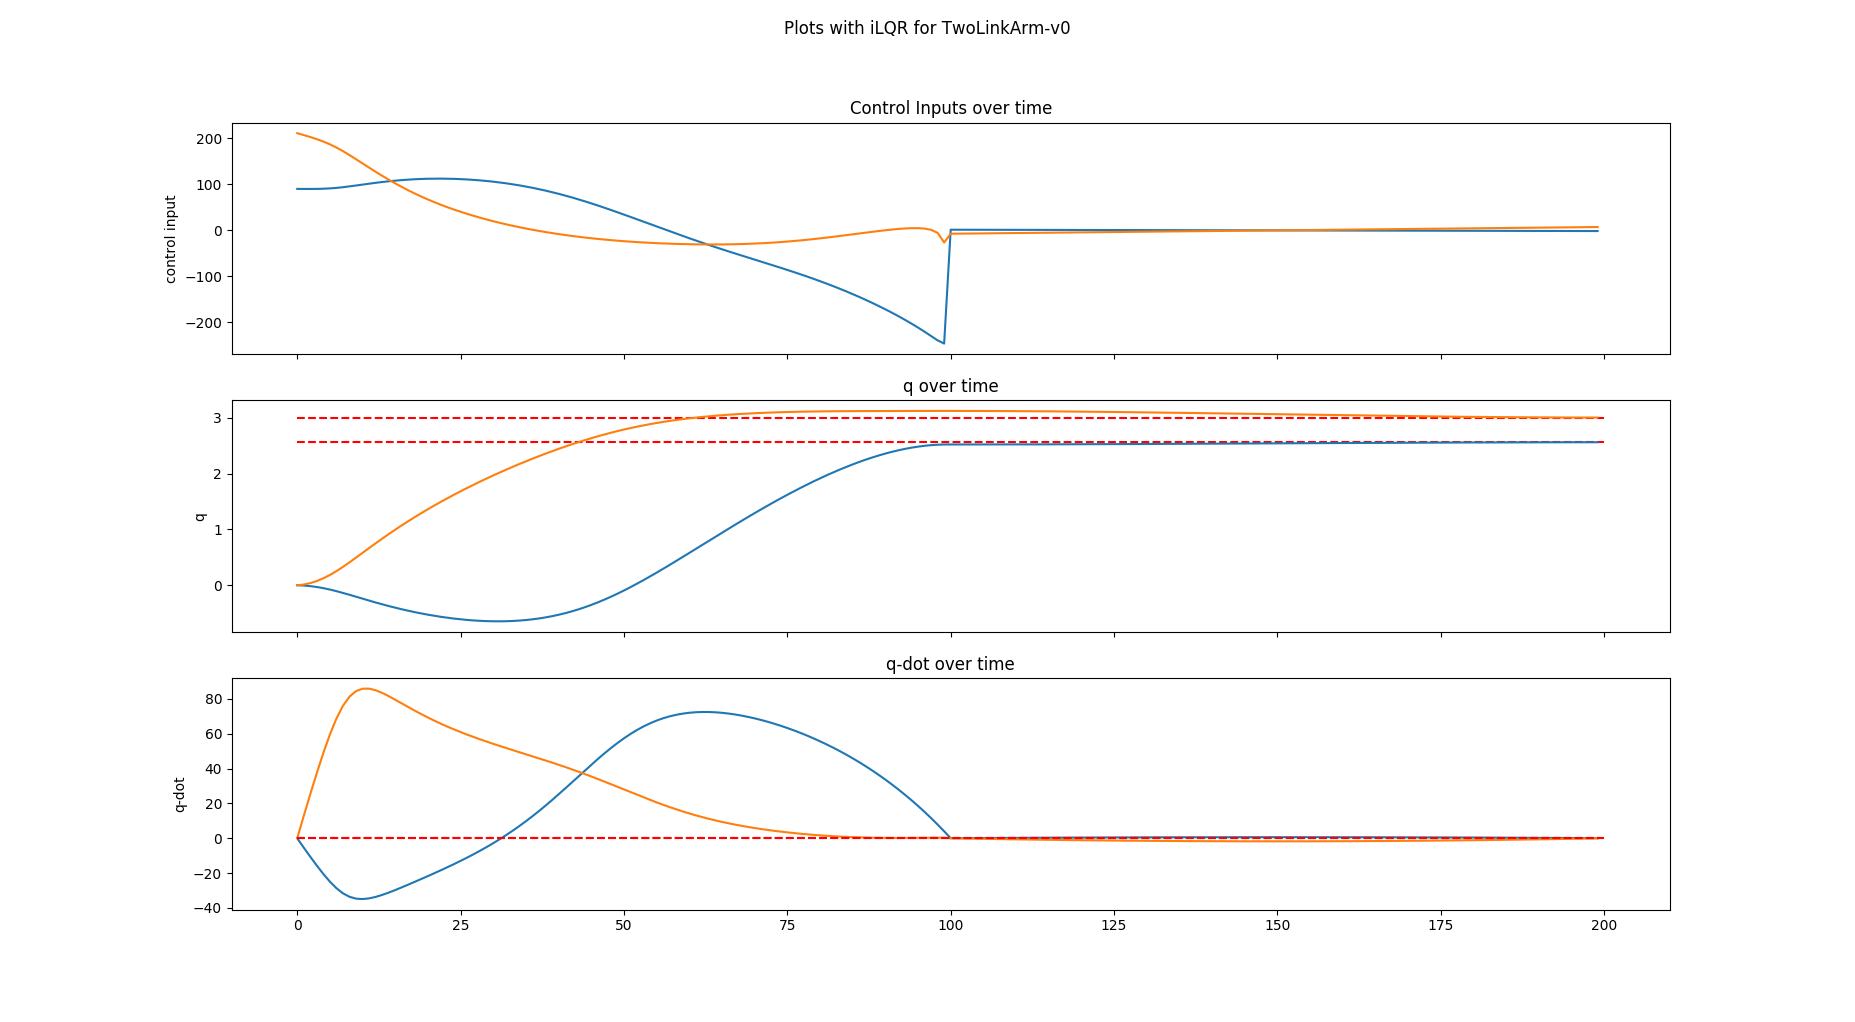
\includegraphics[width=\textwidth]{figures/ilqr_two_link-v0}
        \caption{TwoLinkArm-v0}
    \end{subfigure}
    \begin{subfigure}[b]{0.45\textwidth}
        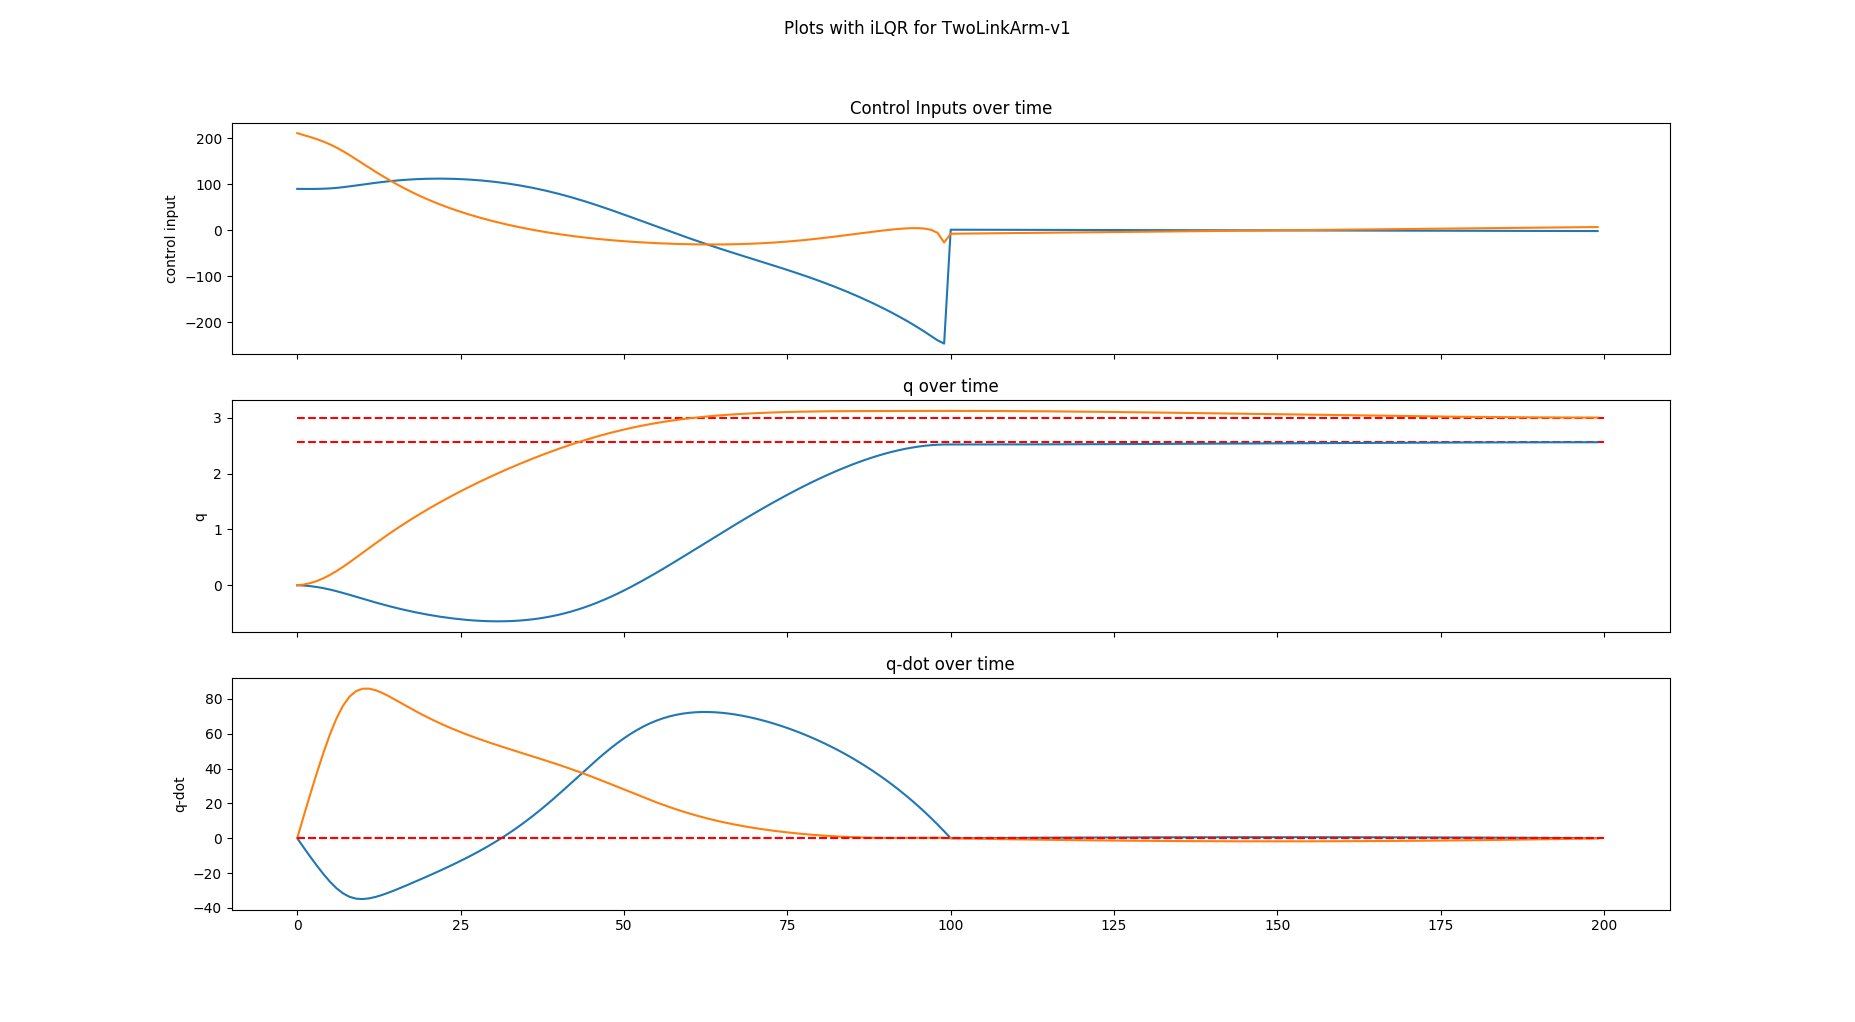
\includegraphics[width=\textwidth]{figures/ilqr_two_link-v1}
        \caption{TwoLinkArm-v1}
    \end{subfigure}
    \caption{Control signals, robot arm state in different environment over time for iLQR}\label{fig:iLQR_state}
\end{figure}
\begin{figure}[H]
	\centering
    \begin{subfigure}[b]{0.45\textwidth}
        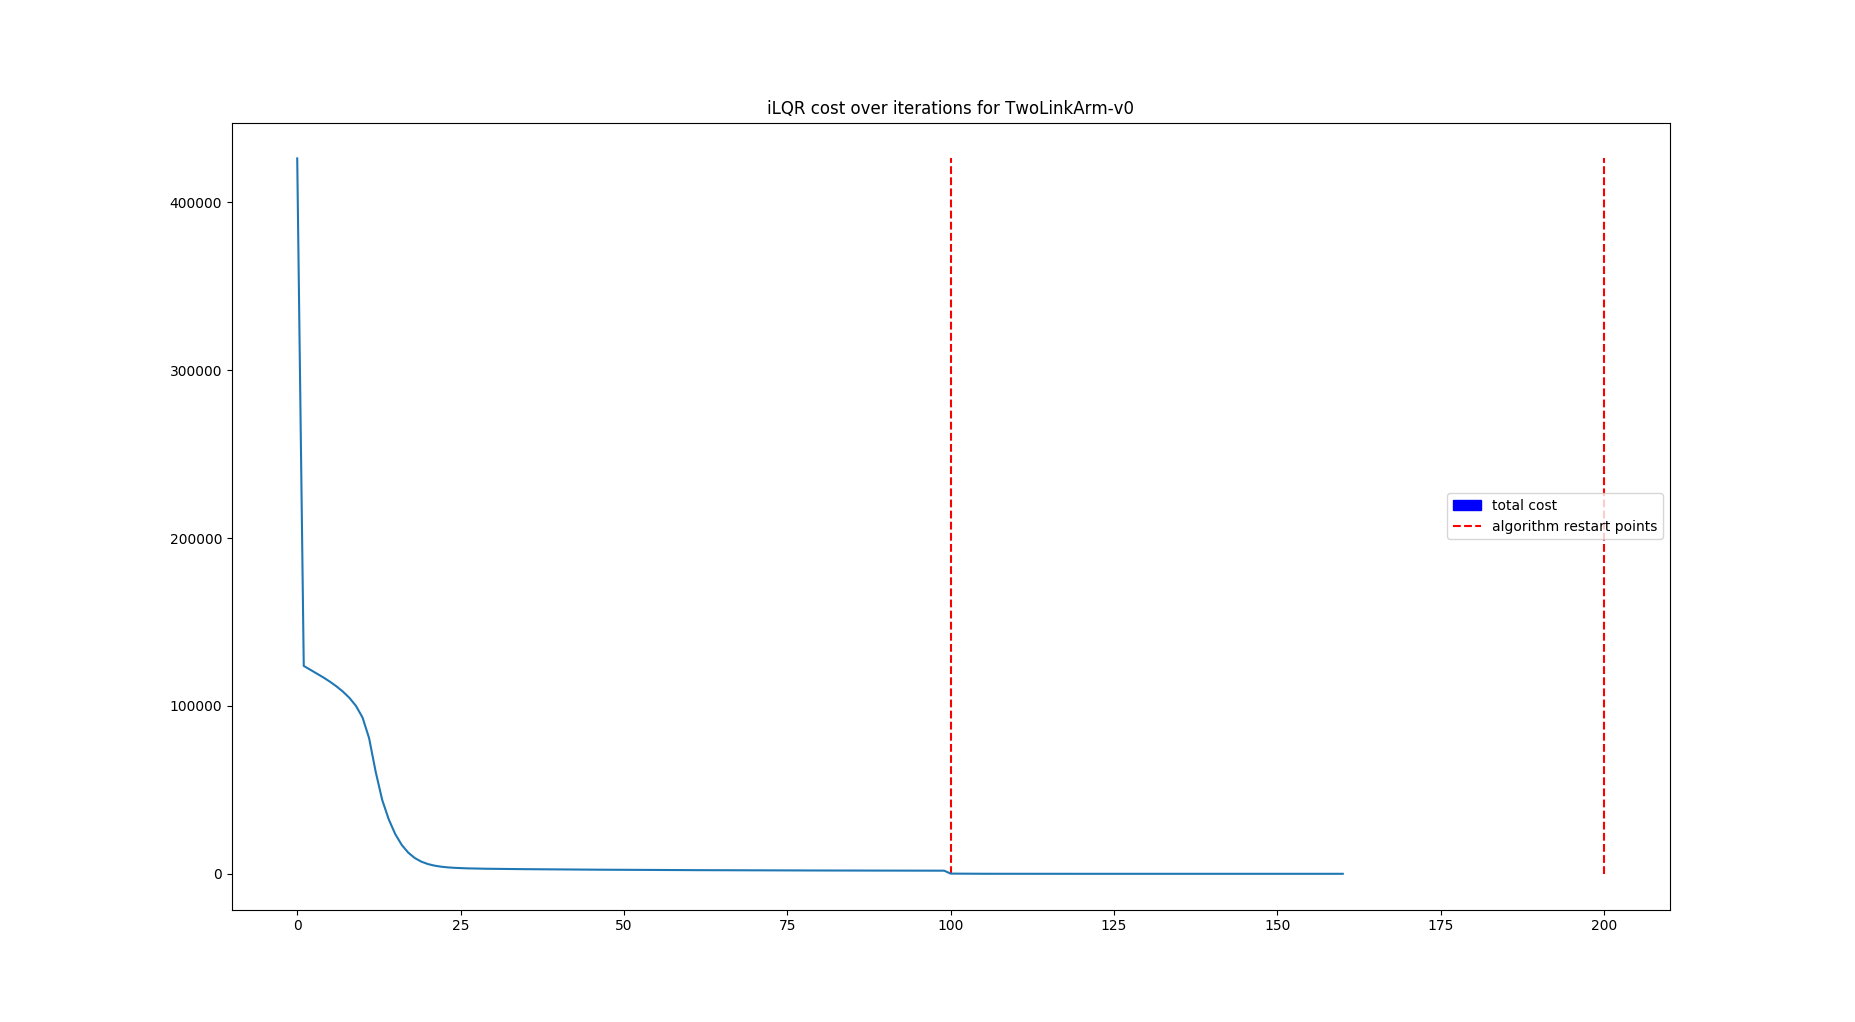
\includegraphics[width=\textwidth]{figures/ilqr2-cost1}
        \caption{TwoLinkArm-v0}
    \end{subfigure}
    \begin{subfigure}[b]{0.45\textwidth}
        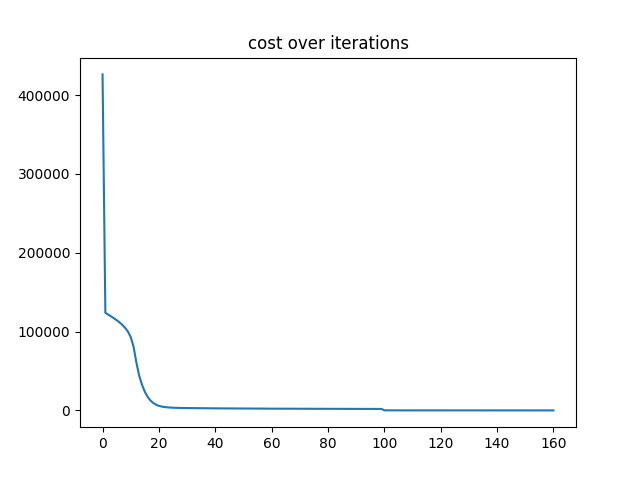
\includegraphics[width=\textwidth]{figures/ilqr2-cost2}
        \caption{TwoLinkArm-v1}
    \end{subfigure}
    \caption{Cost of the calculated path at each iterations. The red dash line denotes when the iLQR algorithm was restarted.}\label{fig:iLQR_cost}
\end{figure}
\subsubsection*{Analysis}
The most obvious difference between iLQR and LQR was the smoothness of control signal. Compared to LQR, iLQR's control signals are smoother and more gradual. iLQR also used less torque compared to LQR. This was demonstrated by the cost in the enviornment \textit{TwoLinkArm-v1} where larger negative reward was incurred for higher torques. iLQR outperformmed LQR by a $1500$. However, the downside of iLQR was that it took significantly longer to run. We also noticed a sudden change in the torques after we restarted the algorithm after the first $100$ signal inputs. There was no difference in terms of number of steps for the system to converge.

%%%%%%%%%%%%%%%%%%%%%%%%%%%%%%%%%%%%%%
\newpage
\section*{Problem 2}

\Lbf{1. Training:}\\
Table \ref{table:imitation_training} reports the binary cross-entropy training loss and accuracy of the cloned model trained on data generated from the expert.
The Adam optimizer was used with a learning rate of 0.00025.
Each cloned model was trained for 50 epochs with a batch size of 32.

Data was generated using different numbers of training samples, generated by recording the state and action of the expert.
The expert always completed the environment until time step 200, when it was terminated.
Thus each episode of training data consists of 200 individual state-action samples.

\begin{table}[h]
  \centering
  \begin{tabular}{| l | c | c | c | c |}
    \hline
    Episodes of Training Data & 1 & 10 & 50 & 100
    \\
    \hline
    Training Loss: & 0.401 & 0.250 & 0.962 & 0.079 \\
    \hline
    Accuracy: & 0.875 & 0.885 & 0.962 & 0.968 \\
    \hline
  \end{tabular}
  \captionof{table}{Loss and accuracy for final training epoch of cloned behavior}
  \label{table:imitation_training}
\end{table}


\Lbf{2. Evaluation on simple environment:}\\
Table \ref{table:imitation_evaluation_easy} reports the cumulative reward averaged over 50 episodes for the cloned behaviors and the Expert on the easier, unwrapped CartPole-v0.
In this environment the maximum reward ever seen is 200.
In this simple environment the cloned behavior with only 1 episode of training data performs worse than the expert, but all other cloned behaviors are able to balance the pendulum to receive the maximum reward.

\begin{table}[h]
  \centering
  \begin{tabular}{| l | c | c | c | c | c |}
    \hline
    Episodes of Training Data & 1 & 10 & 50 & 100 & Expert
    \\
    \hline
    Reward: & 100.18 \pm 33.09 & 200 \pm 0.0 & 200 \pm 0.0 & 200 \pm 0.0 & 200 \pm 0.0\\
    \hline
  \end{tabular}
  \captionof{table}{Cumulative reward for the cloned models and the expert averaged over 50 trails in the basic (unwrapped) CartPole-v0 environment}
  \label{table:imitation_evaluation_easy}
\end{table}


\Lbf{3. Evaluation on the hard environment:}\\
Table \ref{table:imitation_evaluation_hard} reports the cumulative reward averaged over 50 episodes for the cloned behaviors and the Expert on the harder, wrapped CartPole-v0.
In this harder environment all behaviors perform worse compared to the easier environment.
While there is a large improvement for training the cloned behavior on 10 episodes compared to 1 episode, additional training does not help (in the reported trail the averaged total reward actually decreased slightly).
None of the cloned behaviors match the reward of the expert.

\begin{table}[h]
  \centering
  \begin{tabular}{| l | c | c | c | c | c |}
    \hline
    Episodes of Training Data & 1 & 10 & 50 & 100 & Expert
    \\
    \hline
    Reward: & 19.82 \pm 17.62 & 64.80 \pm 58.08 & 51.2 \pm 53.12 & 44.2 \pm 52.12 & 69.8 \pm 50.4 \\
    \hline
  \end{tabular}
  \captionof{table}{Cumulative reward for the cloned models and the expert averaged over 50 trails in the more difficult, wrapped CartPole-v0 environment}
  \label{table:imitation_evaluation_hard}
\end{table}



%%%%%%%%%%%%%%%%%%%%%%%%%%%%%%%%%%%%%%
\newpage
\section*{Problem 3}

\end{document}
